\documentclass[10pt,letterpaper]{article}
\usepackage[T1]{fontenc}
\usepackage[utf8]{inputenc}
\usepackage{libertinus}
\usepackage[margin=0.9in]{geometry}
\usepackage{microtype,booktabs,tabularx,graphicx,xcolor,enumitem,amsmath}
\usepackage[version=4]{mhchem}
\usepackage[font=small,labelfont=bf,skip=4pt]{caption}
\usepackage{titlesec}
\usepackage[hidelinks]{hyperref}
\usepackage{listings}

\definecolor{ink}{HTML}{1B1F24}
\definecolor{sig}{HTML}{C2410C}
\hypersetup{colorlinks,urlcolor=sig!80!black,linkcolor=ink,citecolor=ink}
\titleformat{\section}{\large\bfseries}{\thesection}{0.6em}{}
\titlespacing*{\section}{0pt}{1.1em}{0.35em}
\setlist{nosep,leftmargin=1.2em}
\setlength{\parskip}{0.35em}
\setlength{\parindent}{0pt}
\graphicspath{{../methods/fig/}}
\lstset{basicstyle=\ttfamily\footnotesize,columns=fullflexible,breaklines=true,frame=none,xleftmargin=0.6em}
\newcommand{\Otwo}{\ce{O2}}
\newcommand{\ntrs}[1]{\href{https://ntrs.nasa.gov/citations/#1}{NTRS~#1}}

\begin{document}

{\small\color{ink!70}NASA Space Apps Challenge 2026 \textperiodcentered{} Flame in Freefall \textperiodcentered{} Team Tee to Three}\par\vspace{0.4em}
{\LARGE\bfseries The fire-safety margin Earth tests lose in microgravity,\\ and what it means for Moon-base air\par}
\vspace{0.6em}
{\normalsize Arush Wadhawan \quad Chanatun Kohsuwan}\par
{\small Dashboard \url{https://soulsniper-v2.github.io/flame-in-freefall/}\\ Code and data \url{https://github.com/SoulSniper-V2/flame-in-freefall}\par}
\vspace{0.8em}

\noindent\colorbox{ink!5}{\parbox{\dimexpr\linewidth-2\fboxsep}{\small
\textbf{Abstract.} Apollo~1 showed that the cabin atmosphere decides how dangerous a spacecraft fire is, and the challenge expects Moon-base air at 30\% oxygen or more and 10.2~psia or less. We asked whether NASA's orbital fire-safety evidence covers that air. We combined all 24 combustion investigations in NASA's Physical Sciences Informatics (PSI) database, 1{,}186 test conditions traced to their NASA table cells, and 708 unique measurements that SI extracted from 84 NASA reports, each kept only if its quote appears verbatim in the source. Three results follow. (1)~Using NASA's definition of the oxygen margin of safety, thin films and fabrics burned at 1.2 to 3.9 points lower oxygen in microgravity than in NASA's 1-g screening test; the mean, $-2.6$, matches the value NASA published in 2012. (2)~PSI's ISS solid-material tests stop at 22.2\% \Otwo, so none reaches Moon-base air. (3)~Models trained on 794 measured ISS outcomes predict unseen high-oxygen flights at less than half the naive error with calibrated intervals. The dashboard turns these into a material check, re-test bands for five habitats, SI-written briefs whose numbers are machine-checked, and a recommended next experiment.}}

\section{Question and scope}
NASA screens cabin materials with NASA-STD-6001 Test~1, an upward-burning test at 1\,g. The challenge asks for a tool that summarizes, ranks and interprets PSI combustion data for fire safety in future habitats. We framed one question a mission engineer would ask: \emph{if a material passes the 1-g test for a habitat's air, does it stay safe in reduced gravity, and what evidence exists at that air?} The dashboard covers five habitats: spacecraft cabin and ISS (21\% \Otwo, 14.7~psia, 0\,g), lunar base (30\%, 10.2~psia, 0.166\,g, from the challenge brief), Mars base (same air, 0.38\,g, an assumption) and a pressurized rover (34\%, 8.2~psia, the NASA exploration atmosphere).

\section{Data and provenance}
\textbf{PSI.} We read PSI's public JSON API for all 24 combustion investigations (ACME and its sub-experiments, BASS, BASS-II, Saffire I--III, SAME, SAME-R, DAFT, FLEX, FLEX-2, CFI, SPICE, SLICE and ground studies). 2{,}009 experiment-table rows were parsed into 1{,}186 unit-normalised oxygen and pressure conditions. Every converted value keeps its NASA table, CSV line and verbatim cell, and the dashboard links each point back to it.

\textbf{NASA reports.} 84 open-access reports from the NASA Technical Reports Server and PSI attachments form the literature corpus (\texttt{data/literature/catalog.json}). Flame-spread rates, extinction and flammability limits, ignition times and flame sizes were extracted with their material, oxygen, pressure, gravity, flow and verbatim quote.

\textbf{Measured outcomes for modelling.} 257 FLEX droplet burning-rate measurements, 206 FLEX extinction outcomes and 331 ACME CFI-G ignition attempts: 794 in total.

\section{Literature extraction and its verification firewall}
SI agents proposed literature records. A deterministic script (\texttt{pipeline/lit/verify.py}) accepts a record only if (a)~its quote occurs verbatim in the paper text after whitespace normalisation and (b)~the quote contains the reported number. Each record is labelled by basis using rules on the quote: \textbf{measured} (580), \textbf{cited} from another work (68), \textbf{model} output (41) or \textbf{estimate}, including predictions phrased as ``will be'' (19). In the shipped run 743 candidate rows passed, collapsing to 708 unique records. Only measured values serve as first-hand evidence; the rest are shown with their label. The firewall and the basis rules re-run as unit tests on every build.

\section{The oxygen margin of safety}
NASA/TM-2008-215260 (\ntrs{20080034883}) defines the oxygen margin of safety as the difference between the mean microgravity flammability limit and the mean 1-g limit, using the upward limiting oxygen index (ULOI) and the maximum oxygen concentration (MOC):
\begin{equation}
\mathrm{OMOS} \;=\; \tfrac12\big(\mathrm{ULOI}_{0g}+\mathrm{MOC}_{0g}\big) \;-\; \tfrac12\big(\mathrm{ULOI}_{1g}+\mathrm{MOC}_{1g}\big).
\label{eq:omos}
\end{equation}
We compute it within each report that measured the same material in both gravities, then average across reports. Records with no ignition, pressure above 150~kPa or partial gravity are excluded. Negative values mean the material burns at lower oxygen in microgravity than the 1-g test indicates. The 0-g limits for the thin materials come from NASA Glenn's Zero Gravity Research Facility drop tower.

\begin{figure}[h]
\centering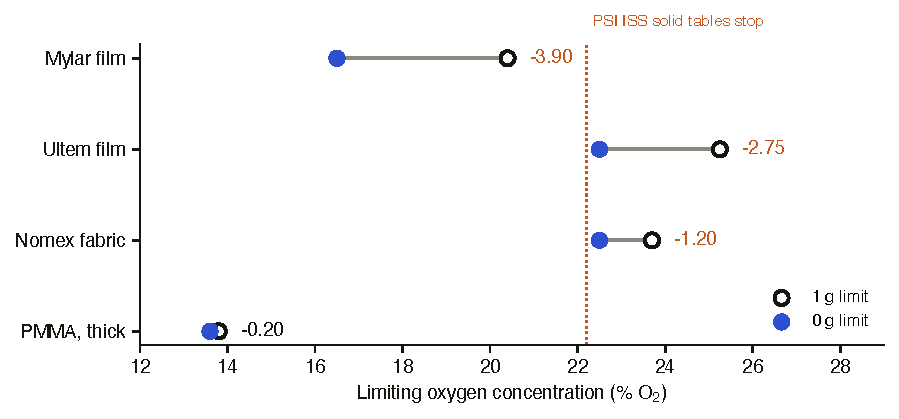
\includegraphics[width=0.92\linewidth]{f1-omos.pdf}
\caption{Limiting oxygen at 1\,g (open) and 0\,g (filled), from quote-verified records (PMMA: zero-stretch 1-g value; see Table~\ref{tab:omos}). The dotted line marks where PSI's ISS solid-material tables stop (22.2\% \Otwo).}
\end{figure}

\begin{table}[h]
\centering\small
\caption{Oxygen margin of safety by material (\% \Otwo).}\label{tab:omos}
\begin{tabularx}{\linewidth}{@{}Xrrrl@{}}
\toprule
Material & 1\,g & 0\,g & OMOS & Source \\
\midrule
Mylar film & 20.4 & 16.5 & $-3.90$ & \ntrs{20080034883} \\
Ultem 1000 film & 25.25 & 22.5 & $-2.75$ & \ntrs{20080034883} \\
Nomex HT90-40 fabric & 23.7 & 22.5 & $-1.20$ & \ntrs{20080034883} \\
\addlinespace
\textbf{Thin-material mean} & & & $\mathbf{-2.62}$ & NASA reported $-2.6$ (\ntrs{20130000677}) \\
\midrule
PMMA rod, 1-g zero-stretch extrapolation & 13.8 & 13.6 & $-0.20$ & 20160012691, 20170006615 \\
PMMA 1/4-in rod, 1-g blowoff vs BASS-II (reported) & 16 & 13.6 & $-2.4$ & \ntrs{20160000593} \\
PMMA rods, SM\textmu RF (reported) & & & $-1.4$ & \ntrs{20200000361} \\
\bottomrule
\end{tabularx}
\par\smallskip\footnotesize\raggedright
Mylar and Ultem were tested at 10.2~psia and Nomex at 14.7~psia, all with 30~cm/s forced flow. Agreement with NASA's $-2.6$ is a consistency check on our extraction and arithmetic, not an independent replication: all three thin materials come from one report. Our PMMA value is small because those 1-g limits are zero-stretch extrapolations; against the 1-g blowoff limit NASA reports $-2.4$, so the material check uses NASA's reported values for thick fuels.
\end{table}

\section{From margin to decision: material check and re-test bands}
A material whose Test~1 limit is $L$ is estimated to burn in reduced gravity at about $L+\mathrm{OMOS}$. For a habitat with oxygen fraction $H$ the dashboard returns
\begin{equation}
\text{verdict}(L,H)=
\begin{cases}
\text{fails at 1\,g} & L \le H,\\
\text{re-test in microgravity} & L > H \ \text{and}\ L+\mathrm{OMOS}_{\text{worst}} \le H,\\
\text{margin holds} & \text{otherwise,}
\end{cases}
\end{equation}
with $\mathrm{OMOS}_{\text{worst}}=-3.9$, the largest thin-material loss measured so far. This gives the re-test bands in Table~\ref{tab:bands}.

\begin{table}[h]
\centering\small
\caption{Re-test bands: materials whose 1-g limit falls in the band pass Test~1 but may burn in microgravity.}\label{tab:bands}
\begin{tabular}{@{}lcc@{}}
\toprule
Habitat & Design \Otwo & Re-test if 1-g limit is between \\
\midrule
Spacecraft cabin, ISS & 21\% & 21.0\% and 24.9\% \\
Lunar base, Mars base & 30\% & 30.0\% and 33.9\% \\
Pressurized rover & 34\% & 34.0\% and 37.9\% \\
\bottomrule
\end{tabular}
\end{table}

\textbf{Leave-one-material-out test.} To see whether the worst-case de-rating generalises, we predicted each thin material's 0-g limit from its 1-g limit and the other two materials' OMOS. The worst-case prediction was conservative for Ultem (21.35 predicted vs 22.5 measured) and Nomex (19.8 vs 22.5) but not for Mylar (17.65 vs 16.5, a 1.15-point miss). Three materials cannot bound the loss, so the dashboard flags materials for testing and does not rate them.

\section{The evidence gap at Moon-base air}
\begin{figure}[h]
\centering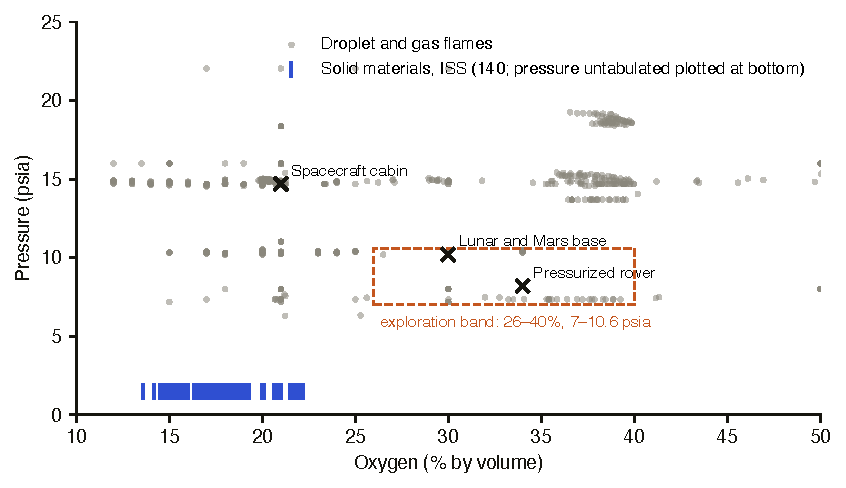
\includegraphics[width=0.92\linewidth]{f2-envelope.pdf}
\caption{Every PSI condition with tabulated oxygen and pressure. Solid-material ISS tests (ticks) tabulate oxygen only and stop at 22.2\%. The exploration band holds 84 conditions, all droplet or gas flames.}
\end{figure}
No solid-material flame in PSI reaches the lunar or rover atmosphere, and PSI holds no partial-gravity combustion data. Outside PSI, the Saffire IV--VI flights on Cygnus burned cotton and PMMA at up to 26.2\% \Otwo{} and about 71~kPa (\ntrs{20210011521}, \ntrs{20240002981}), the closest any solid-material flight test has come; none reached 30\%. LUCI flew material samples at simulated lunar gravity on a spinning New Shepard capsule in 2025 (\ntrs{20250010653}); the verified literature adds its 0.167\,g records, which the dashboard surfaces for lunar and Mars briefs.

\section{What burned on the Space Station: BASS-II outcomes restored}
PSI's BASS-II table lists the conditions of 129 ISS solid-fuel tests (material, oxygen, fan and flow settings) but not their outcomes. Appendix~A of the BASS-II summary report (NASA/TM-20210011385) records a written observation for each test. We parsed the appendix (\texttt{pipeline/bass2/}), recovered 124 observations, joined each to its PSI row by test number, and labelled whether a flame was sustained after the igniter was off. Labels were written by SI from the observation and reviewed against it; 114 are decidable across five materials. Three tests (T9, T10, T12) also appear as ``no ignition'' in an independent NASA paper (\ntrs{20150008962}), in agreement with our labels.

For test $i$ of material $m(i)$ at initial oxygen $x_i$ we fit
\begin{equation}
\Pr(\text{sustained flame}_i)=\sigma\big(\alpha_{m(i)}+\beta\,x_i\big),\qquad
x_{50,m}=-\alpha_m/\beta ,
\end{equation}
with one shared slope $\beta$ and one offset per material; $x_{50,m}$ is the oxygen at a 50\% chance of a sustained flame. Left out one test at a time, the model's Brier score is 0.071 against 0.108 for the base rate (34\% skill). Accuracy is a weak measure here: 100 of the 114 decidable tests burned, so always predicting a burn scores 88\% and the model scores 89\%; the 14 tests that went out carry the fit. Intervals come from 1{,}000 test-level bootstrap resamples. Adding initial flow speed did not improve the held-out Brier score (0.077), so the model has no flow term; this is a limitation, since flow is the second axis BASS-II mapped.

\begin{figure}[h]
\centering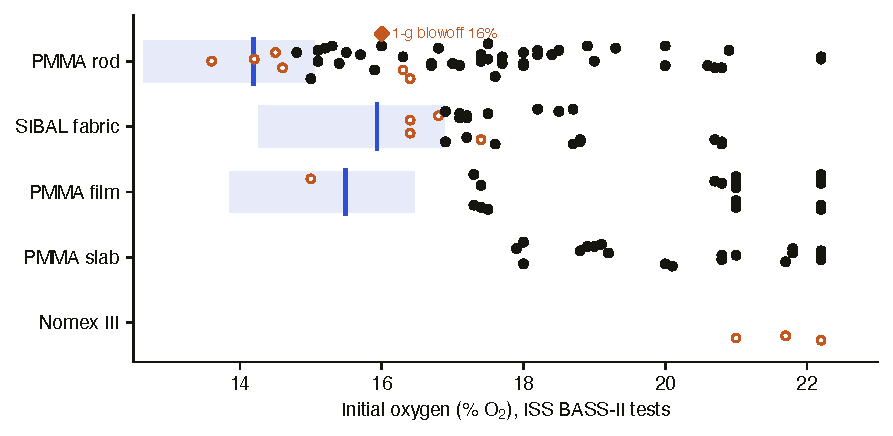
\includegraphics[width=0.92\linewidth]{f4-bass2.pdf}
\caption{Each BASS-II ISS test by material and initial oxygen: filled = sustained flame, open = went out. Line and band: $x_{50}$ with its 90\% interval, shown only for materials that both burned and went out. Diamond: NASA's 1-g blowoff limit for the PMMA rod.}
\end{figure}

\begin{table}[h]
\centering\small
\caption{BASS-II restored outcomes and the oxygen at a 50\% chance of a sustained flame.}\label{tab:bass2}
\begin{tabular}{@{}lrll@{}}
\toprule
Material & Tests & Lowest \Otwo{} that burned & $x_{50}$ (90\% interval) \\
\midrule
PMMA rod, 6--13 mm & 48 & 14.8\% (O4) & 14.2\% (12.6--15.1) \\
SIBAL cotton-fiberglass fabric & 22 & 16.9\% (T14) & 15.9\% (14.3--16.9) \\
PMMA film, 0.1--0.4 mm & 21 & 17.3\% (B16) & 15.5\% (13.8--16.5) \\
PMMA slab, 1--5 mm (all burned) & 20 & 17.9\% (M18) & not identified; below 17.9\% \\
Nomex III fabric (none burned) & 3 & --- & not identified; above 22.2\% \\
\bottomrule
\end{tabular}
\end{table}

The rod result agrees with NASA's own reading of the same data: steady spreading at 13.6\% \Otwo{} against a 1-g blowoff limit of 16\%. Nomex~III not sustaining a flame at 22.2\% matches NASA's 22\% microgravity limit. This is a check of our label restoration against NASA's analysis of the same tests, not an independent result. Flow, sample width and igniter differ between tests, which widens the intervals; the film estimate rests on a single test that went out.

The observations also log where flames went out as the fan was turned down or up: 16 low-flow quench points for PMMA rods and 5 blowoff points. They are in fan-control units with no velocity calibration in PSI, and the quench points sit at nearly the same setting (0.28--0.38) from 14.8\% to 20.0\% \Otwo, which suggests the fan's lowest usable setting rather than a flame limit. We release them in the observation text and do not model them. Five calibrated final-\Otwo{} values cannot be chamber readings (0.6\%, 0.9\%, 1.6\%, 39.1\% and 40.4\%; tests P22a, T28a, B2, P22b and T28b). The same values appear in the report's Appendix~A, and in each case the raw post-burn reading is missing, so they look like a calibration applied to a missing reading rather than a transcription error in PSI. We flag them and do not use them.

\section{Ranking the evidence}
For each investigation an SI extraction, reviewed by the team against its PSI record, scores relevance to prevention $P$, detection $D$, suppression $S$ and modeling $M$ from 0 to 10, each with a one-line rationale tied to a PSI field. Then
\begin{align}
\mathrm{FSI} &= 0.6\,(0.35P+0.25S+0.20D+0.20M) + 0.4\,\max(P,S,D,M),\\
\text{habitat score} &= 0.50\,\mathrm{FSI} + 0.25\,A + 0.10\,G + 0.15\,R,
\end{align}
where $A=e^{-d}$ is the atmosphere match to the nearest tabulated test point, with $d$ in units of 10 \Otwo{} points and 0.3~atm (points that tabulate only oxygen count at 60\%); $G$ is gravity coverage (1.0 for microgravity data in a microgravity habitat, 0.65 otherwise); and $R$ is material realism. Users can change the weights; the brief reports top-five stability under $\pm10$-point changes to any one weight (95\% for the lunar base).

\section{Predictive models and validation}
All models were fitted with scikit-learn on NASA's measured outcomes. Cross-validation was grouped by test day, so no day appears in both training and test folds. Browser copies of the models are unit-tested against scikit-learn outputs.

\begin{table}[h]
\centering\small
\caption{Held-out performance (grouped cross-validation).}\label{tab:models}
\begin{tabularx}{\linewidth}{@{}Xrlll@{}}
\toprule
Model and target & $n$ & Held-out & Baseline & Calibration \\
\midrule
Gaussian process: FLEX droplet burning-rate $K$ (mm$^2$/s) & 257 & $R^2$ 0.672, MAE 0.048 & MAE 0.107 (naive) & 95\% PI covers 92\% \\
Deep ensemble (8 MLPs): FLEX extinction & 206 & AUC 0.834, Brier 0.092 & AUC 0.775 (logistic) & ECE 0.078 \\
Random forest (150 trees): CFI-G hot ignition & 331 & AUC 0.822, Brier 0.120 & Brier 0.137 (logistic) & ECE 0.056 \\
\bottomrule
\end{tabularx}
\end{table}

\begin{table}[h]
\centering\small
\caption{Out-of-distribution tests of the burning-rate model (MAE in mm$^2$/s).}\label{tab:ood}
\begin{tabular}{@{}lrrrr@{}}
\toprule
Split (train $\rightarrow$ test) & $n$ test & MAE & Naive MAE & 95\% coverage \\
\midrule
\Otwo{} $\le 25\%$ $\rightarrow$ \Otwo{} $>25\%$ & 23 & \textbf{0.085} & 0.203 & 96\% \\
$\ge 0.9$~atm $\rightarrow$ lower pressure & 101 & \textbf{0.055} & 0.128 & 98\% \\
no helium $\rightarrow$ helium mixtures & 47 & 0.142 & 0.142 & 96\% \\
\bottomrule
\end{tabular}
\par\smallskip\footnotesize The helium split shows no gain over naive, and its intervals widen to reflect that.
\end{table}

The GP kernel is $1.68^2\cdot\mathrm{RBF}$ with six per-input length scales (2.12 to 6.53) plus white noise 0.196. The extinction ensemble and ignition forest were selected by grouped-CV Brier score against logistic, polynomial-logistic, MLP and gradient-boosting alternatives.

\textbf{Next experiment.} For candidate conditions $c$ from 15\% to 40\% \Otwo{} and 6.6 to 17.6~psia,
\begin{equation}
\text{value}(c)=\sigma_{\text{epi}}(c)\,\big(0.15+\mathrm{rel}(c)\big),
\end{equation}
where $\sigma_{\text{epi}}$ is the GP's epistemic standard deviation and $\mathrm{rel}$ is a Gaussian closeness to the lunar and rover atmospheres, a standard active-learning acquisition rule. The top pick is a 3~mm heptane droplet at 36\% \Otwo{} and 7.7~psia, where predictive uncertainty is 3.5 times that at ISS air.

\section{SI interpretation layer and its firewall}
The challenge asks the tool to interpret, not only to chart. A script (\texttt{si/facts.py}) computes numbered facts for each habitat (H1--H9) and investigation (I1--I7, L1--L3, G1), each with its source. An SI model then writes three sentences per item, citing fact ids. A second script (\texttt{si/verify\_interp.py}) rejects any sentence that cites no fact or an unknown fact, contains a number absent from its cited facts, uses overclaim words (guarantee, certify, proves, always, never, safe to use and similar) or runs over 45 words. 87 sentences across 5 habitats and 24 investigations pass; on the site each citation opens the fact and its source. The same checks run as unit tests.

\section{A negative result: physics-based transfer}
We also tried a physics model: de Ris thin-fuel spread theory with a critical flame temperature, flame temperatures from Cantera, fitted on nitrogen-diluted 1-g spread data by Olson, Stouffer and Grady as tabulated in Friedman (1999), NASA/TM-1999-209285 (\ntrs{19990063738}), and tested on other diluents. It fit nitrogen well but over-predicted helium by about $2.5\times$ (Figure~\ref{fig:phys}), so it is not used on the dashboard. We report it because it marks where simple theory stops being reliable for exploration atmospheres.

\begin{figure}[h]
\centering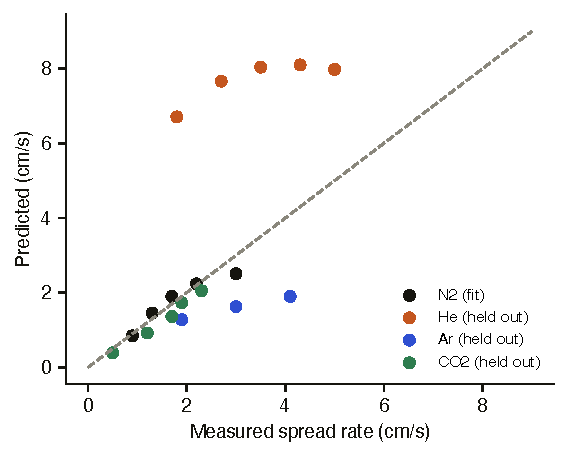
\includegraphics[width=0.55\linewidth]{f3-physics.pdf}
\caption{Thin-fuel spread, measured vs predicted. Fitted on \ce{N2}; held-out He, Ar and \ce{CO2} diluents. Dashed: perfect prediction.}\label{fig:phys}
\end{figure}

\section{Limitations}
\begin{itemize}
\item PSI holds no partial-gravity combustion data; lunar-gravity behaviour is not measured here.
\item The thin-material OMOS rests on three materials from one report, tested with forced flow; the leave-one-out test shows the worst case can be exceeded.
\item The droplet and gas-flame models do not describe solids; the BASS-II burn model covers five solid materials at ISS-like oxygen and 1~atm only.
\item Helium mixtures are predicted no better than the naive baseline; the model widens its intervals accordingly.
\item Scores rank evidence; they do not certify materials. Predictions are for research triage and education.
\item SI-extracted literature values are checked for verbatim quotes, not re-measured. Ranking scores come from SI extractions reviewed by the team, not by combustion experts.
\end{itemize}

\section{Reproducibility}
\begin{lstlisting}
pip install -r pipeline/requirements.txt && ./pipeline/run_all.sh   # PSI API to conditions
python3 pipeline/lit/verify.py                                       # literature firewall
python3 ml/train_models.py                                           # models, metrics.json
python3 si/facts.py && python3 si/verify_interp.py                   # SI interpretation firewall
for s in parse_appendix observations build model; do python3 pipeline/bass2/$s.py; done
cd web && npm ci && npm test && npm run build                        # 27 tests, static site
\end{lstlisting}
Every number in this report is read from the repository's data files; figures come from \texttt{submission/\allowbreak methods/\allowbreak figs.py} and this document from \texttt{submission/\allowbreak report/\allowbreak report.tex}.

\section*{Use of SI}
SI was used to extract structured fields and relevance scores from PSI records (team-reviewed), to propose literature records (accepted only through the quote firewall), to label BASS-II outcomes from NASA's written observations (reviewed, cross-checked), to write interpretation sentences (accepted only through the fact firewall), and to assist with code. The question, method and conclusions came from the team, the challenge text and the PSI data. No SI-generated images are used; flame images are NASA photographs.

\section*{References}
{\small
\begin{enumerate}[label={[\arabic*]},leftmargin=2em,itemsep=2pt]
\item Olson, S.\,L., Ruff, G.\,A., \& Miller, F.\,J. (2008). Microgravity flame spread in exploration atmospheres: pressure, oxygen, and velocity effects on opposed and concurrent flame spread. NASA/TM-2008-215260. \ntrs{20080034883}.
\item Urban, D.\,L., Ruff, G.\,A., Minster, O., et al. (2012). Large scale experiments on spacecraft fire safety. IAC-12. \ntrs{20130000677}.
\item Ferkul, P., Brown, L., Mroczka, C., et al. (2019). Solid Fuel Ignition and Extinction (SoFIE) project on ISS. \ntrs{20200000361}.
\item Friedman, R. (1999). Fire safety in the low-gravity spacecraft environment. NASA/TM-1999-209285. \ntrs{19990063738}.
\item Olson, S.\,L., Ferkul, P.\,V., Bhattacharjee, S., et al. (2021). Burning and Suppression of Solids--II (BASS-II) summary report. NASA/TM-20210011385. \ntrs{20210011385}.
\item NASA Physical Sciences Informatics, combustion investigations, CC0-1.0. \url{https://psi.nasa.gov}; dataset DOIs listed in the repository README.
\item NASA Technical Reports Server, 84 open-access reports (\texttt{data/literature/catalog.json}). NASA-STD-6001B, Flammability, offgassing and compatibility requirements and test procedures.
\item Pedregosa, F., et al. (2011). Scikit-learn: machine learning in Python. \emph{JMLR}, 12, 2825--2830.
\item Goodwin, D.\,G., et al. Cantera. \url{https://cantera.org}.
\end{enumerate}}

\end{document}
